%% LyX 2.1.0 created this file.  For more info, see http://www.lyx.org/.
%% Do not edit unless you really know what you are doing.
\documentclass[a4]{report}
\usepackage[utf8]{inputenc}
\usepackage[tmargin=1cm,bmargin=2cm,lmargin=1cm,rmargin=1cm]{geometry}
\usepackage{multicol}
%-------------------------------------------------------------
% AMS
%-------------------------------------------------------------
\usepackage{amsthm}
\usepackage{amsmath}
\usepackage{amssymb}
%-------------------------------------------------------------

\usepackage{graphicx}
\usepackage[unicode=true,pdfusetitle,
 bookmarks=true,bookmarksnumbered=false,bookmarksopen=false,
 breaklinks=false,pdfborder={0 0 1},backref=false,colorlinks=false]
 {hyperref}

%-------------------------------------------------------------
% Algorithms
%-------------------------------------------------------------
\usepackage{algorithm}
\usepackage{algorithmicx}
\usepackage{algpseudocode}
\usepackage{listings}
\usepackage{color}
\lstset{ %
  %backgroundcolor=\color{white},   % choose the background color; you must add \usepackage{color} or \usepackage{xcolor}
  basicstyle=\footnotesize,        % the size of the fonts that are used for the code
  breakatwhitespace=false,         % sets if automatic breaks should only happen at whitespace
  breaklines=true,                 % sets automatic line breaking
  captionpos=b,                    % sets the caption-position to bottom
  commentstyle=\color{green!30!black},    % comment style
  deletekeywords={...},            % if you want to delete keywords from the given language
  escapeinside={\%*}{*)},          % if you want to add LaTeX within your code
  extendedchars=true,              % lets you use non-ASCII characters; for 8-bits encodings only, does not work with UTF-8
  %frame=single,                    % adds a frame around the code
  keepspaces=true,                 % keeps spaces in text, useful for keeping indentation of code (possibly needs columns=flexible)
  keywordstyle=\color{blue},       % keyword style
  language=Octave,                 % the language of the code
  morekeywords={*,...},            % if you want to add more keywords to the set
  numbers=left,                    % where to put the line-numbers; possible values are (none, left, right)
  numbersep=5pt,                   % how far the line-numbers are from the code
  numberstyle=\tiny\color{gray}, % the style that is used for the line-numbers
  rulecolor=\color{black},         % if not set, the frame-color may be changed on line-breaks within not-black text (e.g. comments (green here))
  showspaces=false,                % show spaces everywhere adding particular underscores; it overrides 'showstringspaces'
  showstringspaces=false,          % underline spaces within strings only
  showtabs=false,                  % show tabs within strings adding particular underscores
  stepnumber=2,                    % the step between two line-numbers. If it's 1, each line will be numbered
  stringstyle=\color{purple},     % string literal style
  tabsize=2,                       % sets default tabsize to 2 spaces
  title=\lstname                   % show the filename of files included with \lstinputlisting; also try caption instead of title
}
%-------------------------------------------------------------

%-------------------------------------------------------------
% glossaries
%-------------------------------------------------------------
\usepackage[acronym]{glossaries}
\newacronym{LSR}{LSR}{least squares regression}
\newacronym{SISO}{SISO}{Single-input-single-output}
\newacronym{LTI}{LTI}{Linear time-invariant}
\newacronym{ISE}{ISE}{Integral Square error}
\newacronym[longplural=ordinary differential equations]{ODE}{ODE}{ordinary differential equation}
\newacronym[longplural=Algebraic Ricatti Equations]{ARE}{ARE}{Algebraic Ricatti equation}
\makeglossaries
%-------------------------------------------------------------

\makeatletter

%%%%%%%%%%%%%%%%%%%%%%%%%%%%%% Textclass specific LaTeX commands.
\theoremstyle{plain}
\newtheorem{thm}{\protect\theoremname}
\theoremstyle{definition}
\newtheorem{defn}[thm]{\protect\definitionname}
\theoremstyle{plain}
\newtheorem{fact}[thm]{\protect\factname}
\theoremstyle{plain}
\newtheorem{prop}[thm]{\protect\propositionname}
\ifx\proof\undefined
\newenvironment{proof}[1][\protect\proofname]{\par
\normalfont\topsep6\p@\@plus6\p@\relax
\trivlist
\itemindent\parindent
\item[\hskip\labelsep\scshape #1]\ignorespaces
}{%
\endtrivlist\@endpefalse
}
\providecommand{\proofname}{Proof}
\fi

%%%%%%%%%%%%%%%%%%%%%%%%%%%%%% User specified LaTeX commands.
%-------------------------------------
% tikz
%-------------------------------------
\usepackage{tikz}
%-------------------------------------

%-------------------------------------
% breqn
%-------------------------------------
\usepackage{breqn}
% Add support for automatic equation breaking
\gdef\wrap@breqn@environ#1#2{
    \expandafter\let\csname breqn@oldbegin@#1\expandafter\endcsname\csname #1\endcsname
    \expandafter\let\csname breqn@oldend@#1\expandafter\endcsname\csname end#1\endcsname
    \expandafter\gdef\csname breqn@begin@#1\endcsname{%
        \expandafter\let\csname #1\expandafter\endcsname\csname breqn@oldbegin@#1\endcsname%
        \begin{#2}%
    }
    \expandafter\gdef\csname breqn@end@#1\endcsname{%
        \expandafter\let\csname end#1\expandafter\endcsname\csname breqn@oldend@#1\endcsname%
        \end{#2}%
        \expandafter\let\csname #1\expandafter\endcsname\csname breqn@begin@#1\endcsname%
        \expandafter\let\csname end#1\expandafter\endcsname\csname breqn@end@#1\endcsname%
    }
    \expandafter\let\csname #1\expandafter\endcsname\csname breqn@begin@#1\endcsname
    \expandafter\let\csname end#1\expandafter\endcsname\csname breqn@end@#1\endcsname
}
\wrap@breqn@environ{equation}{dmath}
\wrap@breqn@environ{equation*}{dmath*}
%-------------------------------------

%-------------------------------------
% easy macros
%-------------------------------------
\newcommand\pdev[2]{\dfrac{\partial #1}{\partial #2}}
%-------------------------------------

\makeatother

\providecommand{\definitionname}{Definition}
\providecommand{\factname}{Fact}
\providecommand{\propositionname}{Proposition}
\providecommand{\theoremname}{Theorem}
\renewcommand{\lstlistingname}{Listing}

\begin{document}
\global\long\def\R{\mathbb{R}}
\global\long\def\N{\mathbb{N}}
\global\long\def\Z{\mathbb{Z}}
\global\long\def\Q{\mathbb{Q}}

\title{Activity Log}

\author{Rodolfo Jordao}

\maketitle
\tableofcontents{}

\listofalgorithms

\listoffigures

\listoftables

\printglossaries

\chapter{Modelling}

\section{Kinematics}

\subsection{Angles and Positions dependence:}

\begin{figure}[h]
\begin{center}
\begin{tikzpicture}[scale=2]
\draw (0,0) circle (1cm) node (C1) {$C_2$};
\draw +(2,1) circle (0.8cm) node (C2) {$C_1$};
\draw (C1) -- ++(150:0.7cm) node (P1) {} node[below left,midway] {$d_2$};
\draw (C2) -- ++(110:0.5cm) node (P2) {} node[left,pos=0.4] {$d_1$};
\draw (P2) -- (P1) node[midway,above] {$L_1$};
\draw[dashed] (C2) |- (C1) node[pos=0.25,right] {$d_y$} node[pos=0.7,below] {$d_x$};
%theta2
\draw[dashed] (60:-0.7cm) -- (C1) -- (60:0.7cm);
\draw[dashed] (60:0.6cm) arc (60:0:0.6cm) node[midway,right] {$\theta_2$};
%theta1
\draw[dashed] (C2) -- +(0.6cm,0);
\draw[dashed] (C2) -- ++(110:0.4cm) arc (110:0:0.4cm) node[midway,right] {$\theta_1$};
\end{tikzpicture}
\end{center}
\caption{First sketch. \label{fig:first:sketch.}}
\end{figure}

From Fig.~\ref{fig:first:sketch.},
\begin{align*}
L_{1}c_{3}-d_{2}s_{2}-d_{1}c_{1} & =d_{x}\\
L_{1}s_{3}+d_{2}c_{2}-d_{1}s_{1} & =d_{y}
\end{align*}
rearrange to isolate the pseudo angle,
\begin{align*}
L_{1}c_{3} & =d_{x}+d_{2}s_{2}+d_{1}c_{1}\\
L_{1}s_{3} & =d_{y}-d_{2}c_{2}+d_{1}s_{1}
\end{align*}
square both equations and sum them,
\[
L_{1}^{2}=d_{x}^{2}+d_{y}^{2}+d_{1}^{2}+d_{2}^{2}+2\left(d_{x}d_{2}s_{2}+d_{x}d_{1}c_{1}+d_{1}d_{2}c_{1}s_{2}-d_{y}d_{2}c_{2}+d_{y}d_{1}s_{1}-d_{1}d_{2}s_{1}c_{2}\right)
\]
for simplicity, let,
\begin{align*}
K & =\frac{L_{1}^{2}-\left(d_{x}^{2}+d_{y}^{2}+d_{1}^{2}+d_{2}^{2}+2d_{x}d_{1}c_{1}+2d_{y}d_{1}s_{1}\right)}{2}\\
a & =d_{x}d_{1}+d_{1}d_{2}c_{1}\\
b & =-(d_{y}d_{2}+d_{1}d_{2}s_{1})
\end{align*}
giving,
\[
K=as_{2}+bc_{2}
\]
then,
\begin{align*}
c_{2} & =\frac{bK+\sqrt{b^{2}K^{2}-\left(a^{2}+b^{2}\right)\left(K^{2}-a^{2}\right)}}{a^{2}+b^{2}}\\
 & =\frac{bK+a\sqrt{a^{2}+b^{2}-K^{2}}}{a^{2}+b^{2}}
\end{align*}
finally,
\[
\theta_{2}=Atan2\left(\sqrt{1-c_{2}^{2}},c_{2}\right)
\]

\begin{figure}[h]
\begin{center}
\begin{tikzpicture}[scale=2.0]
\node (C) at (0,0) {$C_1$};
\coordinate (P) at (0.3cm,-1.5cm);
\draw (0,0) circle (1cm);
\draw (C) -- +(30:0.6cm) node[midway,above] {$d_3$} -- (P) node[midway,right] {$L_2$};
\draw[dashed] ++(30:0.6cm) -- ++(30:0.1cm) arc (30:0:0.7cm) node[midway,right] {$\theta_2$} --+(-0.1,0);
\draw[dashed] (C) |- (P) node[pos=0.25,left] {$y_1$} node[pos=0.8,below] {$a_1$};
\draw[dashed] (C) -- (P) ;
\draw[dashed] (P) -- ++(82:0.4cm) arc (82:0:0.4cm) node[midway,right] {$\theta_3$} --cycle;
\end{tikzpicture}
\end{center}
\caption{Second Sketch.}
\end{figure}

\begin{align*}
a_{1}+L_2\cos \theta_3 & =d_{3}\cos\theta_{2}\\
d_{3}\sin\theta_{2}+y_{1} & =L_{2}\sin\theta_{3}
\end{align*}
rearranging these equations:
\begin{align*}
L_2\cos \theta_3 & =d_{3}\cos\theta_{2} -a_1 \\
L_{2}\sin\theta_{3}&= y_{1}+ d_{3}\sin\theta_{2}
\end{align*}
these can be squared and summed to give:
\[
y_{1}^{2}+2y_{1}d_{3}s_{2}+s_{2}^{2}d_{3}^{2}-L_{2}^{2}+\left(d_{3}c_{2}-a_1\right)^{2}=0
\]
getting the roots:
\[
y_{1}=-d_{3}s_{2}+\sqrt{L_2^2-(a_1-d_3c_2)^2}
\]
the same reasoning can be applied to get $y_2$.

\subsection{Best linearization candidate}
\label{sec:best:lin:candidate}

Since most of the operational routine the system will oscillate about
$\theta_{2}=0$, a good candidate for linearization of the system
should be the values of $\theta_{1}$ which results in this condition.
For this, it is possible to use all equations developed in direct
Kinematics. So the starting equation to solve for $\theta_{1}$ is:
\[
L_{1}^{2}=d_{x}^{2}+d_{y}^{2}+d_{1}^{2}+d_{2}^{2}+2\left(d_{x}d_{1}c_{1}-d_{y}d_{2}+d_{y}d_{1}s_{1}-d_{1}d_{2}s_{1}\right)
\]
\[
\therefore\frac{L_{1}^{2}-\left(d_{x}^{2}+d_{y}^{2}+d_{1}^{2}+d_{2}^{2}\right)}{2}+d_{y}d_{2}=d_{x}d_{1}c_{1}+d_{1}\left(d_{y}-d_{2}\right)s_{1}
\]
making the following simplifications,
\begin{align*}
W & =\frac{L_{1}^{2}-\left(d_{x}^{2}+d_{y}^{2}+d_{1}^{2}+d_{2}^{2}\right)}{2}+d_{y}d_{2}\\
h & =d_{x}d_{1}\\
g & =d_{1}\left(d_{y}-d_{2}\right)
\end{align*}
the solution for $\theta_{1}$ is acquired,
\[
c_{1}=\frac{hW+g\sqrt{g^{2}+h^{2}-W^{2}}}{g^{2}+h^{2}}
\]
\[
s_{1}=\frac{gW-h\sqrt{g^{2}+h^{2}-W^{2}}}{g^{2}+h^{2}}
\]
\[
\theta_{0}=Atan2\left(\sqrt{1-c_{1}^{2}},c_{1}\right)
\]
where $\theta_{0}$ is the angle chosen to lienarize the whole system
about.

\subsection{Localization of all points of interest}

Looking at Fig.~\ref{fig:photo} and assuming that everything has
homogeneous distribution, which can safely be switched later on (even
more assuming that most or all links have axial homogeneity):

\begin{figure}[h]
\begin{center}
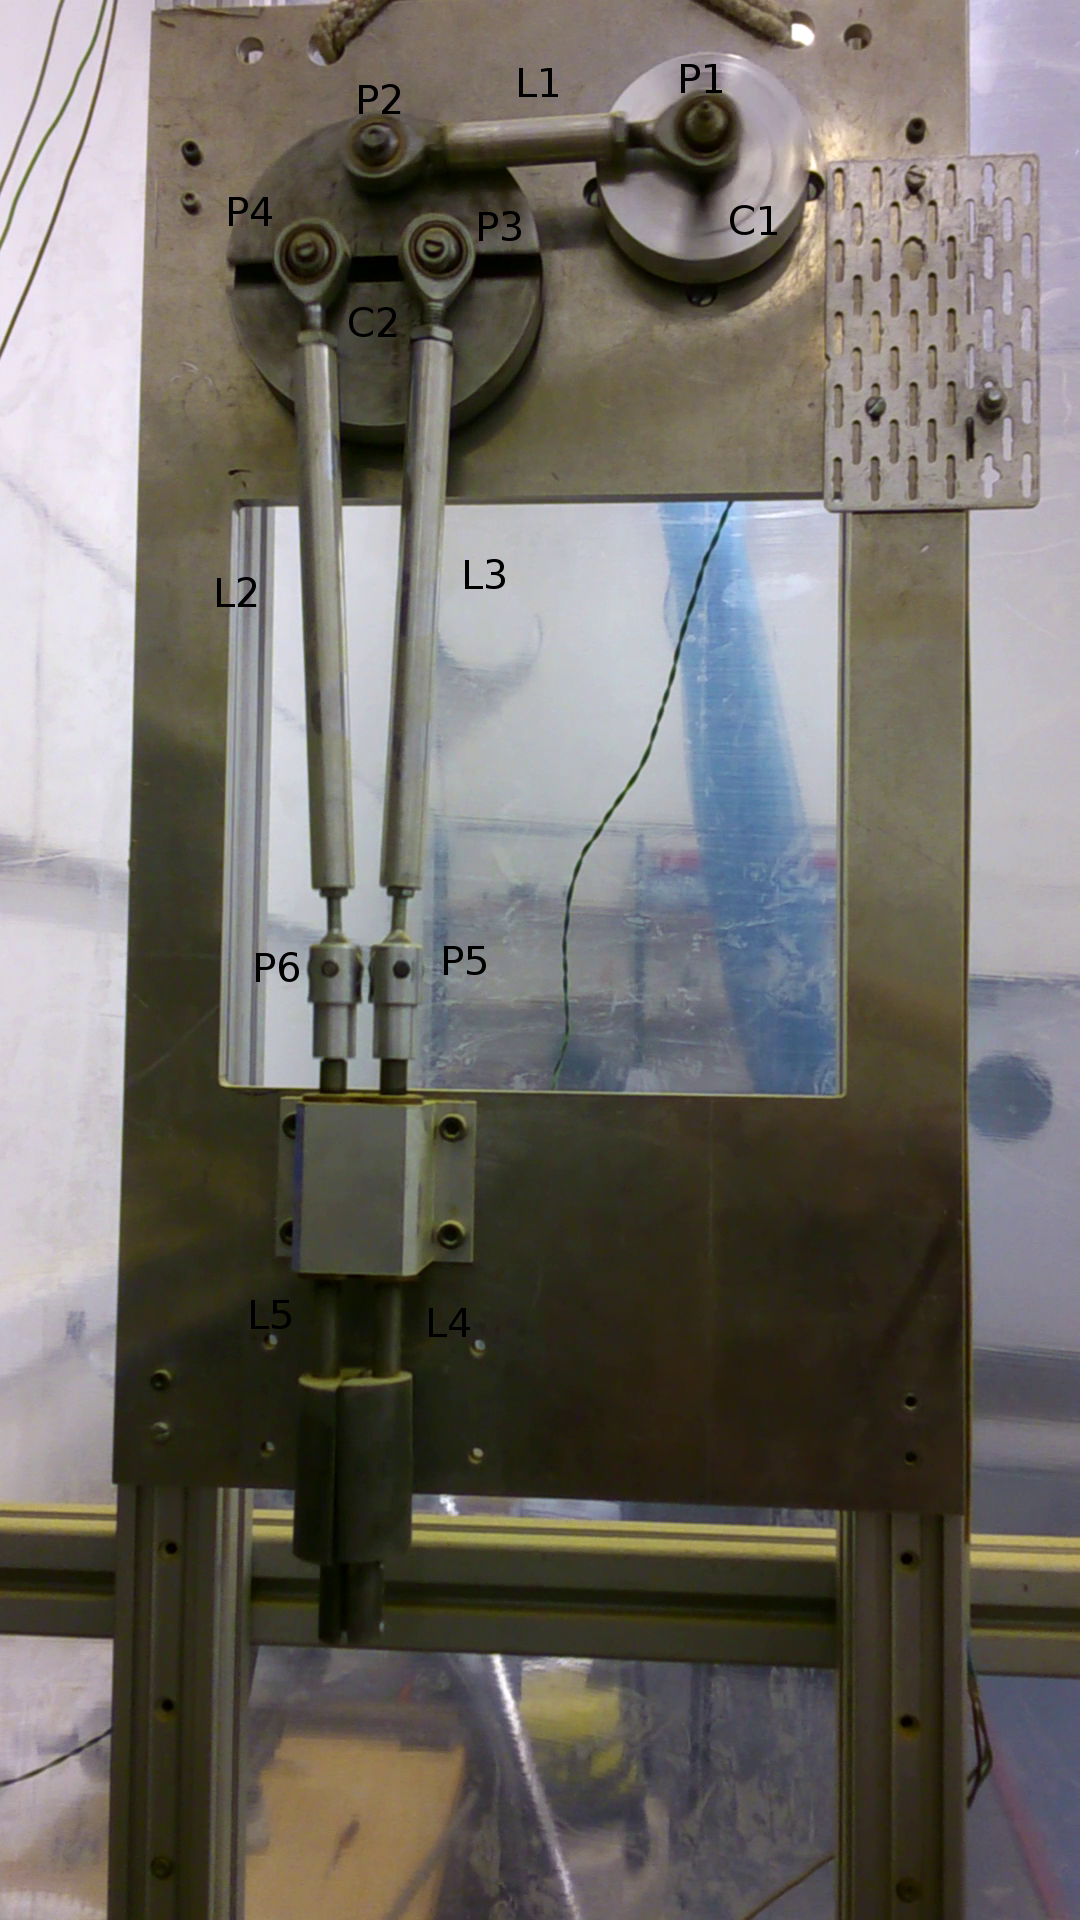
\includegraphics[width=0.35\textwidth]{snapshot}
\end{center}
\caption{Photo of test rig indicating points. \label{fig:photo}}
\end{figure}

\begin{multicols}{2}
\begin{enumerate}
  \item $\mathbf{r}_{C_{1}}=\left(0,0\right)$
  \item $\mathbf{r}_{C_{2}}=\left(c_{x},c_{y}\right)$
  \item $\mathbf{r}_{P_{1}}=\mathbf{r}_{C_{2}}+\left(d_{1}\cos\theta_{1},d_{1}\sin\theta_{1}\right)$
  \item $\mathbf{r}_{P_{2}}=\left(d_{2}\sin\theta_{2},d_{2}\cos\theta_{2}\right)$
  \item $\mathbf{r}_{P_{3}}=\frac{1}{2}\left(d_{3}\cos\theta_{2},d_{3}\sin\theta_{2}\right)$
  \item $\mathbf{r}_{P_{4}}=-\frac{1}{2}\left(d_{4}\cos\theta_{2},d_{4}\sin\theta_{2}\right)$
  \item $\mathbf{r}_{P_{5}}=\left(a_{1},-y_{1}\right)$
  \item $\mathbf{r}_{P_{6}}=\left(a_{2},-y_{2}\right)$
  \item $\mathbf{r}_{L_{1}}=\frac{1}{2}\left(\mathbf{r}_{P_{1}}+\mathbf{r}_{p_{2}}\right)$
  \item $\mathbf{r}_{L_{2}}=\frac{1}{2}\left(\mathbf{r}_{P_{4}}+\mathbf{r}_{P_{6}}\right)$
  \item $\mathbf{r}_{L_{3}}=\frac{1}{2}\left(\mathbf{r}_{P_{3}}+\mathbf{r}_{P_{5}}\right)$
  \item $\mathbf{r}_{L_{4}}=\mathbf{r}_{P_{5}}+\frac{1}{2}\left(0,-L_{4}\right)$
  \item $\mathbf{r}_{L_{5}}=\mathbf{r}_{P_{6}}+\frac{1}{2}\left(0,-L_{5}\right)$\end{enumerate}
\end{multicols}

\subsection{Velocities of all points of interest}

This is necessary for dynamical formulation. Actually it is enough
to differentiate every point localization with respect to time, the
only another requirement is the angular velocity of every body, which
are:
\begin{multicols}{2}
  \begin{enumerate}
    \item $\omega_{C_{1}}=\omega_{P_{1}}=\dot{\theta}_{1}$
    \item $\omega_{C_{2}}=\omega_{P_{2}}=\omega_{P_{3}}=\omega_{P_{4}}=\dot{\theta}_{2}$
    \item $\omega_{L_{1}}={\displaystyle -\frac{\frac{d_{1}s_{2}\dot{\theta}_{1}\dot{\theta}_{2}-d_{2}c_{1}\dot{\theta}_{1}}{d_{1}c_{1}+d_{1}s_{2}+c_{x}}+\frac{{\left(d_{1}c_{2}\dot{\theta}_{1}\dot{\theta}_{2}-d_{1}s_{1}\dot{\theta}_{1}\right)}{\left(d_{1}c_{2}+d_{2}s_{1}+c_{y}\right)}}{{\left(d_{1}c_{1}+d_{1}s_{2}+c_{x}\right)}^{2}}}{\frac{{\left(d_{1}c_{2}+d_{2}s_{1}+c_{y}\right)}^{2}}{{\left(d_{1}c_{1}+d_{1}s_{2}+c_{x}\right)}^{2}}+1}}$
    \item $\omega_{L_{2}}={\displaystyle \frac{\frac{{\left(d_{4}s_{2}-y_{2}\left(\theta_{1}\left(t\right)\right)\right)}d_{4}s_{2}\dot{\theta}_{1}\dot{\theta}_{2}}{{\left(d_{4}c_{2}+a_{2}\right)}^{2}}+\frac{d_{4}c_{2}\dot{\theta}_{1}\dot{\theta}_{2}-\dot{\theta}_{1}\dot{y_{2}}}{d_{4}c_{2}+a_{2}}}{\frac{{\left(d_{4}s_{2}-y_{2}\left(\theta_{1}\left(t\right)\right)\right)}^{2}}{{\left(d_{4}c_{2}+a_{2}\right)}^{2}}+1}}$
    \item $\omega_{L_{3}}={\displaystyle \frac{\frac{{\left(d_{3}s_{2}-y_{1}\left(\theta_{1}\left(t\right)\right)\right)}d_{3}s_{2}\dot{\theta}_{1}\dot{\theta}_{2}}{{\left(d_{3}c_{2}+a_{1}\right)}^{2}}+\frac{d_{3}c_{2}\dot{\theta}_{1}\dot{\theta}_{2}-\dot{\theta}_{1}\dot{y_{1}}}{d_{3}c_{2}+a_{1}}}{\frac{{\left(d_{3}s_{2}-y_{1}\left(\theta_{1}\left(t\right)\right)\right)}^{2}}{{\left(d_{3}c_{2}+a_{1}\right)}^{2}}+1}}$
  \end{enumerate}
\end{multicols}

Also, the rotation of the screws (Every $P$) can possibly be ignored
as it \emph{may} cuase little contribution to the overall system dynamics
if neglected as rigid bodies.

\section{Dynamics}

The symbolic calculations are just too gigantic to fill in one paper.
I made many assumptions that simplified the model but that still did not
make it small enough, I'll try other things. The sagemath code in
Sec.~\ref{sec:sagemath} basically does that.

\subsection{plant model}

the Lagrangian has the form:
\[
L = \sum\frac{m_i}{2}\left(\dot r_i(\theta_1)\right)^2 +\frac{I_i}{2} (\omega_i(\theta_1,\dot \theta_1))^2
-m_i r_i(\theta_1) g
\]
seeing that $\forall i, \omega_i(\theta_1,\dot\theta_1) = \Omega(\theta_1)\dot{\theta_1}$, then:
\begin{align*}
L &= \sum\frac{m_i}{2}\left(\frac{r_i(\theta_1)}{d\theta_1}\right)^2\dot \theta_1^2 +
\frac{I_i}{2} (\Omega_i(\theta_1))^2\dot{\theta_1}^2-m_i r_i(\theta_1) g \\
 &= \dot{\theta_1}^2\left[\sum\frac{m_i}{2}\left(\frac{r_i(\theta_1)}{d\theta_1}\right)^2 +
 \frac{I_i}{2} (\Omega_i(\theta_1))^2\right]-\sum m_i r_i(\theta_1) g
\end{align*}
if the element enclosed in brackets is denominated $V$ while the sum $U$, then:
\[
L = \dot{\theta_1}^2V(\theta_1) - U(\theta_1)
\]
where the equation of motion, disregarding for now outside influence and friction, can be derived:
\begin{align*}
\tau &= \frac{d}{dt}\left(\frac{\partial L}{\partial \dot\theta_1}\right) - \frac{\partial L}{\partial \theta_1} \\
&= \ddot{\theta_1}(2V(\theta_1)) + \dot{\theta}_1^2\frac{dV(\theta_1)}{d\theta_1} + \frac{dU(\theta_1)}{d\theta_1}
\end{align*}
or written more compactly:
\begin{equation}
\tau = 2\ddot{\theta}_1V(\theta_1) + \dot{\theta}_1^2 V'(\theta_1) + U'(\theta_1)
\label{eq:sys:eq:motion}
\end{equation}
finally giving it into more familiar form:
\begin{align}
\begin{split}
\dot \theta_1 &= \omega_1 \\
\dot \omega_1 &= -\omega_1^2 \frac{V'(\theta_1)}{2V(\theta_1)} - \frac{U'(\theta_1)}{2V(\theta_1)} + \frac{\tau}{2V(\theta_1)}
\end{split}
\label{eq:dyn:sys}
\end{align}


\subsection{linearised plant model}

the linear model basically consists into the jacobian of Sys.~\eqref{eq:dyn:sys} evaluated about
equilibrium point discussed in Sec.~\ref{sec:best:lin:candidate}. First define:
\begin{align*}
g(\omega_1,\theta_1)&=-\omega_1^2 \frac{V'(\theta_1)}{2V(\theta_1)} - \frac{U'(\theta_1)}{2V(\theta_1)} \\
f(\omega_1,\theta_1,\tau) &= \frac{\tau}{2V(\theta_1)}
\end{align*}
then clearly, the linearisation will be given by:
\begin{align*}
  \dot\theta_1 &= \pdev{\omega_1}{\theta_1}\theta_1  + \pdev{\omega_1}{\omega_1}\omega_1 \\
  \dot\omega_1 &= \left[\pdev{g}{(\theta_1,\omega_1)}(\theta_0)\right]
  \left[
    \begin{array}{c}
      \theta_1-\theta_0 \\ \omega_1
    \end{array}
  \right]
  +\left[\pdev{f}{(\theta_1,\omega_1)}(\theta_0)\right]
  \left[
    \begin{array}{c}
      \tau \\ \tau
    \end{array}
  \right]
\end{align*}
where the partial is in fact a gradient. These in turn can be written as,
\begin{align}
  \begin{split}
    \dot\theta_1 &= \omega_1 \\
    \dot\omega_1 &= a_1\theta_1 + b_1\omega_1 + c_1 + d_1\tau
  \end{split}
  \label{eq:lin:dyn:sys}
\end{align}
where the coefficients are, symbolically:
\begin{align*}
a_1&=\left[-\omega_1^2\left(\frac{V(\theta_1)V''(\theta_1)-\left(V'(\theta_1)\right)^2}{2V(\theta_1)}\right)
-\left(\frac{V(\theta_1)U''(\theta_1)-V'(\theta_1)U'(\theta_1)}{2V(\theta_1)}\right)
\right]_{\theta_1=\theta_0,\omega_1=0} \\
b_1 &= \left[-\omega_1\frac{V'(\theta_1)}{V(\theta_1)}\right]_{\theta_1=\theta_0,\omega_1=0} \\
c_1 &= -a_1\theta_0 \\
d_1 &= a_1+b_1
\end{align*}
by the chosen equilibrium point, some simplifications can be made:
\begin{align*}
a_1&=-\left(\frac{V(\theta_0)U''(\theta_0)-V'(\theta_0)U'(\theta_0)}{2V(\theta_0)}\right) \\
b_1 &= 0 \\
c_1 &= -a_1\theta_0 \\
d_1 &= a_1+b_1
\end{align*}

An even better way to linearise this sytem is to look into Eq.~\eqref{eq:sys:eq:motion},
and make this the starting equation, since this can easily then give the linearised
torque the motor should generate. First, see that the torque is function of three
independent variables: $\theta,\omega,\dot\omega$, thus:
\[
\nabla\tau = \left(\frac{\partial \tau}{\partial \theta},\frac{\partial \tau}{\partial \omega},\frac{\partial \tau}{\partial \dot\omega}\right)
\]
seeing that $x_0 = (\theta_0,0,0)$ is the equilibrium point, the sought equation for along the torque will be:
\[
\tau = \left. \nabla\tau \right|_{x=x_0} \left[
\begin{array}{c}
  \theta-\theta_0 \\
  \omega \\
  \dot \omega
\end{array}
\right]
\]
or expanded in explicit form,
\begin{align}
  \tau &= \left(2V'(\theta_0)\right)\dot\omega
  +\left(2\omega_0V'(\theta_0)\right)\omega+\left(2\dot\omega_0V'(\theta_0)+\omega_0^2V''(\theta_0)+U''(\theta_0)\right)(\theta-\theta_0) \nonumber \\
  \therefore\tau &= 2V'(\theta_0)\dot\omega + U''(\theta_0)(\theta-\theta_0)
  \label{eq:sys:lin:eq:motion}
\end{align}

\subsection{overall model}

It can be found easily in the internet or elsewhere that the coupled \glspl{ODE} modelling
the motor's behaviour are given by:
\begin{align*}
  \dot i &= -\frac{R}{L}i - \frac{k_e}{L}\omega_m + \frac{1}{L}V_s \\
  \dot \omega_m &= \frac{k_t}{J}i - \frac{k_e}{J} + \frac{1}{J}\tau_m
\end{align*}
these can be combined with the previous equation of motion developed for the drill rig:
\begin{align*}
  \dot i &= -\frac{R}{L}i - \frac{k_e}{L}\omega_m + \frac{1}{L}V_s \\
  \dot \omega_m &= \frac{k_t}{J}i - \frac{k_e}{J}\omega_m + \frac{1}{J}\frac{1}{N}\left(a\dot\omega_o+b\omega_o+c\theta_o+d\right) \\
  \dot \theta_m &= \omega_m
\end{align*}
finally noting that $N\theta_0 = \theta_m$:
\[
  \dot \omega_m = \frac{k_t}{J}i - \frac{k_e}{J}\omega_m + \frac{1}{J}\frac{1}{N^2}\left(a\dot\omega_m+b\omega_m+c\theta_m+d\right)
\]
\[
  \left(1-\frac{a}{N^2}\right) \dot \omega_m = \frac{k_t}{J}i +\left(\frac{b}{JN^2}-\frac{k_e}{J}\right)\omega_m
  +\frac{c}{JN^2}\theta_m+\frac{d}{JN^2}
\]
finally, the overall linearized system coupled \glspl{ODE} can be written:
\begin{align}
  \begin{split}
  \dot i &= -\frac{R}{L}i - \frac{k_e}{L}\omega_m + \frac{1}{L}V_s \\
  \dot \omega_m &= \frac{N^2k_t}{J(N^2-a)}i + \frac{1}{J}\left(\frac{b-N^2k_e}{N^2-a}\right)\omega
  + \frac{c}{J(N^2-a)}\theta + \frac{d}{J(N^2-a)} \\
  \dot \theta_m &= \omega_m
  \end{split}
  \label{eq:sys:lumped:lti}
\end{align}
using $x=(i,\omega,\theta)$, the standard form for dynamical systems:
\[
x = Ax + BV_s + Ex_o
\]
where:
\def\A{
\left[
\begin{array}{ccc}
  -\frac{R}{L} & \frac{k_e}{L} & 0 \\
  \frac{N^2k_t}{J(N^2-a)} & \frac{1}{J}\left(\frac{b-N^2k_e}{N^2-a}\right) & \frac{c}{J(N^2-a)} \\
  0 & 1 & 0
\end{array}
\right]}
\def\B{
\left[
\begin{array}{c}
  \frac{1}{L} \\
  0 \\
  0
\end{array}
\right]}
\def\E{\left[
\begin{array}{c}
  0 \\
  \frac{d}{J(N^2-a)} \\
  0
\end{array}
\right]}
\[
A = \A
\]
\[
B = \B
\]
\[
E = \E
\]

\section{Control Measures}
\subsection{Inicial considerations}
The main goal is to control the reciprocating frequency, which can make use of the
efficient internal loop of the controller into the system.
the IxR methodology to account for  voltage drop is given in Fig.~\ref{fig:overall:diag}.
\begin{figure}[h]
\begin{center}
	\begin{tikzpicture}
\tikzstyle{Circle} = [draw,font={\huge\bfseries}, shape=circle, minimum size=0.5cm, text=black, very thick, text width=0.2cm, align=center]
\tikzstyle{Dot} = [draw, fill, shape=circle, minimum size=0.2cm]
\tikzstyle{Block} = [draw,outer sep=1,inner sep=2,minimum size=24,line width=1, very thick]
\tikzstyle{inv} = [outer sep=0,inner sep=0,minimum size=0]
\node [Block] (v1) at (-7,3.5) {$\frac{1}{k\times n}$};
\node [Circle] (v2) at (-5,3.5) {};
\node [inv] (v8) at (4.5,0.5) {};
\node [inv] (v9) at (4.5,1.5) {};
\node [inv] (v4) at (-2,3.5) {};
\node [Block] (v5) at (-0.5,3.5) {$T_l(U,i,\omega)$};
\node [Block] (v6) at (2.5,3.5) {$f_{\omega}(\tau,\omega,\theta)$};
\node [inv] (v3) at (4.5,2.5) {};
\node [Block] (v7) at (-1,-1.5) {Arduino};
\node [Block] (v10) at (3.5,1.5) {$\int$};
\node [Block] (v12) at (1.5,-0.5) {$\frac{1}{k\times n}$};
\node [inv] (v11) at (4.5,-0.5) {};
\node [Circle] (v13) at (-2,-0.5) {};
\node [Block] (v15) at (-3.5,-0.5) {R est.};
\node [Dot] (v14) at (-3.5,2) {};
\node [Block] (v16) at (-5,1) {$i\times R$};
\draw [->] (v1) edge node[midway,above] {$U_r$} (v2);
\draw [->] (v2) edge (v5);
\draw [->] (v5) edge node[midway,above] {$\tau$} (v6);
\draw (v6) -| (v3) node[pos=0.2,above] {$\omega$};
\draw [->] (v9) -- (v8) -| (v5.-50);
\draw [->] (v8) -- (v11) -- (v12);
\draw [->] (v12) edge node[pos=0.95,below] {$-$} node[midway,above] {$U_{EMF}$} (v13);
\draw [->] (v4) edge (v13);
\draw [->](v3) -- (v9) -- (v10);
\draw [->] (v3) -| (v6.-40);
\draw [->] (v10) -| (v6.-120);
\draw [->] (v14) edge node[pos=0.2,right] {$i$} (v15);
\draw [->] (v14) |- (v16);
\draw [->] (v15) -| (v16) node[pos=0.3,below] {$R$};
\draw [->] (v16) edge node[midway,left] {$U_{i\times R}$} (v2);
\draw [->] (v13) edge (v15);
\draw [->] (v11) |- (v7);
\draw [->] (v7) -| (v1)  node[below,pos=0.1] {$\omega_r$};
\draw [->] (v14) -| (v5.-140);
\end{tikzpicture}
    
	\caption{Overall diagram showing internal voltage drop control "IxR methodology".
	Every summation point is positive unless noted otherwise.}
	\label{fig:overall:diag}
\end{center}
\end{figure}
The reciprocating motion is dictated by the equation:
\[
y(t) = f(\theta_2(\theta_1(t)))
\]
the period of $y(t)$ is then given by the time elapsed between two equal values of $y$ for
different time. Since this is true for the period of $\theta_1$, it comes that the period $p$
of reciprocation is the same as the period of rotation:
\[
y(t+p) = f(\theta_2(\theta_1(t+p))) = f(\theta_2(\theta_1(t))) = y(t)
\]
Thus the reciprocating frequency is given by:
\[
\frac{f_y}{2\pi} =  \omega_1
\]
If the values for the maximum and minimum heights in each stroke is required, their
deduction follows:
\[
\dot{y} = 0 = \frac{df}{d\theta_2}\frac{d\theta_2}{d\theta_1}\omega_1
\]
since the maxima of $f$ and $\theta_2$ occur at the same points for
their respective variables, it is enough to solve for:
\[
\frac{df(\theta_2)}{d\theta_2} = 0
\]
this is given by:
\[
-d_{{3}}\cos \left( \theta_2 \right) +{\frac { \left( d_{{3}}\cos
	\left( \theta_2 \right) -a_{{1}} \right) d_{{3}}\sin \left( \theta_2
	\right) }{\sqrt {{L_{{2}}}^{2}- \left( d_{{3}}\cos \left( \theta_2
	\right) -a_{{1}} \right) ^{2}}}}=0
\]
which has solutions (along two more):
\[
c_2 = \pm\frac{a_1}{L_2+d_3}
\]
which can be substituted back onto $y(\theta_2)$ to give its maxima and minima:
\begin{align*}
y_m &= \frac{L_2-d_3}{L_2+d_3}\sqrt{\left(L_2^2+d_3^2\right)-a_1^2} \\
y_m^* &= -d_{{3}}\sqrt {1-{\frac {{a_{{1}}}^{2}}{ \left( L_{{2}}+d_{{3}}
			\right) ^{2}}}}+\sqrt {{L_{{2}}}^{2}- \left( -{\frac {d_{{3}}a_{{1}}}
		{L_{{2}}+d_{{3}}}}-a_{{1}} \right) ^{2}}
\end{align*}

\subsection{Optimal gain calculation}

The system, although being defined in three dimensional state space is \gls{SISO}.
Moreover the applied linearization rendered the lumped parameter model \eqref{eq:sys:lumped:lti} \gls{LTI},
thus the classical approach via frequency analysis is readily avaiable for use.

In Eq.~\eqref{eq:sys:lumped:lti}, its laplace transform
is given by:
\begin{align*}
  si &= a_{11}i + a_{12}\omega + bV_s \\
  s\omega &= a_{21} + a_{22}\omega + a_{23}\theta + D \\
  s\theta &= \omega
\end{align*}
where $a_{ij} = \left[A\right]_{ij}$, for simplicty of notation.
Manipulating the first and third of these and substituting into the second:
\[
s\omega = \frac{a_{12}\omega+bV_s}{s-a_{11}} + a_{22}\omega + \frac{a_{23}}{s}\omega + D
\]
which gives:
\[
\left(s-\frac{a_{12}}{s-a_{11}}-a_{22}-\frac{a_{23}}{s}\right)\omega = bV_s + D
\]
or, into a rational form:
\[
\left(\frac{s^3-(a_{11}+a_{22})s^2+(a_{11}a_{22}-a_{12}-a_{23})s+a_{11}a_{23}}{s(s-a_{11})}\right)\omega
=bV_s + D
\]
As $D$ depends upon the choice of initial conditions, and since any of them make the physical
system stable, it can be assumed that $D=0$. Then the transfer function of the overall system:
\begin{equation}
G(s) = \frac{\omega}{V_s} =
\left(\frac{bs(s-a_{11})}{s^3-(a_{11}+a_{22})s^2+(a_{11}a_{22}-a_{12}-a_{23})s+a_{11}a_{23}}\right)
\label{eq:sys:trans:func}
\end{equation}
If the numerical data is used:
\[
G(s) = \input{../SSC-Math/Transfer_function_system.txt}
\]
The controller in question is a PI-like controller,
hence its equation can be assumed to be:
\begin{equation}
  C(s) = K_p\left(1+\frac{1}{T_i s}\right)
\end{equation}
where $K$ and $T_i$ are constants well defined in literature.
The overall closed-loop transfer function changes to:
\[
H(s) = \frac{C(s)G(s)}{1+C(s)G(s)}
\]
or numerically:
\[
H(s) = \input{../SSC-Math/Transfer_function_total.txt}
\]
If a \gls{ISE} is defined as:
\begin{equation}
  I_c = \int_{0}^{\infty}(x(t)-y(t))^2+\sigma^2 u^2dt
  \label{eq:ise}
\end{equation}
where $u$ is the control variable, then Parseval's theorem can be used to
calculate this integral by knowing the transfer functions if each variable.
Therefore, it is necessary to minimize:
\[
I_c = \frac{1}{2\pi}\int_{-\infty}^{\infty}\left(V_s(i\xi)-\omega(i\xi)\right)\left(V_s(-i\xi)-\omega(-i\xi)\right)
+\sigma^2 U(i\xi)U(-i\xi)d\xi
\]
where $i$ is the imaginary unit. It is desirable to manipulate
the integrand before hand of computing the integral, as to minimize the effort required:
\[
\left[V_s(s)-H(s)V_s(s)\right]\left[V_s(-s)-H(-s)V_s(-s)\right]
+\sigma^2 V_s(s)C(s)C(-s)V_s(-s)
\]
assuming that the voltage is an unity step input $1/s$
to prioritize reducing errors in the system,
\[
-\frac{1}{s^2}\left[1-H(s)\right]\left[1-H(-s)\right]
-\sigma^2 \frac{1}{s^2}C(s)C(-s)
\]
as it is expected from the linearizations performed and computed transfer
functions, $H(s)=N_h(s)/D_h(s)$ while $C(s)=N_c(s)/D_c(s)$, therefore:
\[
\left[1-H(s)\right]\left[1-H(-s)\right] + \sigma^2 C(s)C(-s) =
\left[1-\frac{N_h(s)}{D_h(s)}\right]\left[1-\frac{N_h(-s)}{D_h(-s)}\right]
 + \sigma^2 \frac{N_c(s)}{D_c(s)}\frac{N_c(-s)}{D_c(-s)} =
\left[\frac{D_h(s)-N_h(s)}{D_h(s)}\right]\left[\frac{D_h(-s)-N_h(-s)}{D_h(-s)}\right]
 + \sigma^2 \frac{N_c(s)}{D_c(s)}\frac{N_c(-s)}{D_c(-s)} =
\left[\frac{(D_h(s)-N_h(s))D_c(s)}{D_h(s)D_c(s)}\right]\left[\frac{(D_h(-s)-N_h(-s))D_c(-s)}{D_h(-s)D_c(-s)}\right]
 + \sigma^2 \frac{N_c(s)D_h(s)}{D_c(s)D_h(s)}\frac{N_c(-s)D_h(-s)}{D_c(-s)D_h(-s)} =
\left[\frac{(D_h(s)-N_h(s))D_c(s)+\sigma N_c(s)D_h(s)}{D_h(s)D_c(s)}\right]
\left[\frac{(D_h(-s)-N_h(-s))D_c(-s)+\sigma N_c(-s)D_h(-s)}{D_h(-s)D_c(-s)}\right]
\]
if for $\alpha_{abi}$ what is meant is the $i$-th coordinate of $A_b(s)$ polynomial,
it follows from the foregoing calculation that the total polynomials are:
\[
\left(\sum_{i=0}^3(\alpha_{dhi}-\alpha_{nhi})s^i\right)\sum_{j=0}^3\alpha_{dcj}s^j
+ \sigma \left(\sum_{i=0}^1\alpha_{nci}s^i\right)\left(\sum_{j=0}^1\alpha_{dhj}s^j\right)
\]
which is equal to the polynomial
\[
\sum_{i=0}^3\sum_{j=0}^1\left[(\alpha_{dhi}-\alpha_{nhi})\alpha_{dcj}+\sigma \alpha_{nci}\alpha_{dhj}\right]s^{i+j}
\]
giving the total coefficient for each power of s. The denominator deduction is similar
and easier:
\[
\sum_{i=0}^3\sum_{j=0}^1\alpha_{dhi}\alpha_{dcj}s^{i+j}
\]
resulting in a proper rational polynomial of fith order in both,
these calculations can be done with aid of tables or purely solving a linear
system associated with Eq.~\eqref{eq:ise}. These, in turn, can be minimized as factors of each
gain component, that is, $K_p$ and $T_i$, giving a set of two equations to be
solved in respect of these same variables.
\section{Algorithms for Tuning}

\subsection{Theory and Deductions}

After trying the implemented a stall detection algorithm which tried
to exhaust some sequence properties and test them in the Arduino,
they showed no promise. It has become clear that something a little
more sophisticated, however possible of on-line implementation; emulating
maybe a short-term memory was necessary. Certainly the current flowing through the
motor can give good hints upon stalling, but no before prior knowledge
of the system the motor will effectively drive; thus focus
at the feedback speed is the most general option. Using the same fundamental
definitions as before:
\begin{defn}[Stall]
The positive definite error function $e(t)$ is said to be \emph{stalling
about $L$} if there is $\epsilon,t_{o}\in\R$ such that $\forall t>t_{0},\left|e(t)-L\right|<\epsilon$.
In words, the error $e(t)$ is \emph{stalling} if it oscillates (ou
stabilizates) about some value $L$. The discrete version is similar.
\end{defn}
Once again, the same fundamental fact that connect a mathematical
test to the physical problem is stated:
\begin{fact}
if the error function $e(t)$ is not strictly monotonic decreasing,
it is either stalling on some value or increasing.
\end{fact}
This can be proved without too much difficulty. Now, the test that
can be used is that of linear \gls{LSR} of a certain amount of values.
If $n$ error values are sampled giving the vector $\mathbf{e}=\left\{ e_{1},\dots,e_{n}\right\} $
for the following time vector $\mathbf{t}=\left\{ T,\dots,nT\right\} $.
But since the check is for a non-strictly decreasing function, the
vector $\mathbf{t}$ can be simplified to $\mathbf{t}_{c}=\left\{ 1,\dots,n\right\} $.
The reason for so is given by the following:
\begin{defn}
Let $a,b\in\R$ be such that,
\[
e(t)=at+b
\]
is the best approximation of the sampled data $\mathbf{e}=\left\{ e_{1},\dots,e_{n}\right\} $
upon time vector $\mathbf{t}=\left\{ t_{1},\dots,t_{n}\right\} $.
Then $a$ is denominated \emph{trend} of the data and $b$ \emph{start}
of the data. Moreover, these are given by:
\begin{align*}
a & =\frac{n\left(\sum_{i=1}^{n}e_{i}t_{i}\right)-\left(\sum_{i=1}^{n}e_{i}\right)\left(\sum_{i=1}^{n}t_{n}\right)}{n\left(\sum_{i=1}^{n}t_{i}^{2}\right)-\left(\sum_{i=1}^{n}t_{i}\right)^{2}}\\
b & =\frac{\left(\sum_{i=1}^{n}t_{i}^{2}\right)\left(\sum_{i=1}^{n}e_{i}\right)-\left(\sum_{i=1}^{n}e_{i}t_{i}\right)\left(\sum_{i=1}^{n}t_{n}\right)}{n\left(\sum_{i=1}^{n}t_{i}^{2}\right)-\left(\sum_{i=1}^{n}t_{i}\right)^{2}}
\end{align*}

\end{defn}
Since the micro controller samples at approximately a constant interval,
the time vector can be considered $\mathbf{t}=\left\{ T,\dots,nT\right\} $,
and the test for non strictly decreasing function follow:
\begin{prop}[\gls{LSR} test]
Let the error function $e(t)$ be sampled with time vector $\mathbf{t}=\left\{ T,\dots,nT\right\} $.
If the trend obtained by using as a time vector $\mathbf{t}_{c}=\left\{ 1,\dots,n\right\} $
is non-negative, then $e(t)$ cannot be monotonic decreasing.\end{prop}
\begin{proof}
First, a connection between both time vectors is established; let
$a_{1}$ be the trend with $\mathbf{t}$ and $a_{2}$ be the trend
with $\mathbf{t}_{c}$. Then,
\[
a_{1}=\frac{n\left(\sum_{i=1}^{n}e_{i}iT\right)-\left(\sum_{i=1}^{n}e_{i}\right)\left(\sum_{i=1}^{n}iT\right)}{n\left(\sum_{i=1}^{n}iT^{2}\right)-\left(\sum_{i=1}^{n}iT\right)^{2}}=\frac{1}{T}\left[\frac{n\left(\sum_{i=1}^{n}e_{i}i\right)-\left(\sum_{i=1}^{n}e_{i}\right)\left(\sum_{i=1}^{n}i\right)}{n\left(\sum_{i=1}^{n}i^{2}\right)-\left(\sum_{i=1}^{n}i\right)^{2}}\right]=\frac{1}{T}a_{2}
\]
that is, both trends are related by a constant, nominally $1/T$.
To prove the incompatibility between strictly monotonic decreasing
and the trend non-negativity, let $e(t)$ be a strictly monotonic
decreasing function; then its trend with time $\mathbf{t}_{c}$,
\begin{align*}
a & =\frac{n\left(\sum_{i=1}^{n}e_{i}i\right)-\left(\sum_{i=1}^{n}e_{i}\right)\left(\sum_{i=1}^{n}i\right)}{n\left(\sum_{i=1}^{n}i{}^{2}\right)-\left(\sum_{i=1}^{n}i\right)^{2}}\\
 & =\frac{n\left(\sum_{i=1}^{n}e_{i}i\right)-\left(\sum_{i=1}^{n}e_{i}\right)\frac{n}{2}\left(n+1\right)}{n\left(\sum_{i=1}^{n}i{}^{2}\right)-\left(\sum_{i=1}^{n}i\right)^{2}}\\
 & =\frac{\sum_{i=1}^{n}e_{i}\left(ni-n\frac{\left(n+1\right)}{2}\right)}{n\left(\sum_{i=1}^{n}i{}^{2}\right)-\left(\sum_{i=1}^{n}i\right)^{2}}
\end{align*}
since the denominator is a constant, focus is given to the numerator.
By assumption,
\begin{align*}
\sum_{i=1}^{n}e_{i}\left(ni-n\frac{\left(n+1\right)}{2}\right) & <e_{1}\sum_{i=1}^{n}\left(ni-n\frac{\left(n+1\right)}{2}\right)\\
 & =e_{1}\left(\sum_{i=1}^{n}ni-n^{2}\frac{\left(n+1\right)}{2}\right)\\
 & =e_{1}\left(n\left(n\frac{(n+1)}{2}\right)-n^{2}\frac{\left(n+1\right)}{2}\right)\\
 & =0
\end{align*}
while the denominator is positive by using the cauchy-schwarz inequality
with sequences $\left\{ i\right\} _{i}$ and $\left\{ 1\right\} _{i}$.
Since trends with both time vectors are multiple, it is true that
sampling with $\mathbf{t}$ must also give a negative trend. This
completes the proof.
\end{proof}
All formalities aside, a regression test for data is useful as to
determine the possibility of stalling. The implementation is given
in Secs.~\ref{chap:arduino:source}~and~\ref{sec:stall:detection}.

\subsection{Online update improvement}

After some more familiarization with these topics, I've improved
all formulas to the point in making its implementation real-time;
that is, tweaking these estimations to make it recursive. For the sake of
understandability, Define a placeholder for multiplicative sums as follows:
\[
s_{x_1x_2\dots x_m}(n) = \sum_{i=1}^n\left(\prod_{j=1}^mx_{ij}\right)
\]
then, it is possible to generate an updating factor for the linear regression
parameters as follows. let $D(n)=ns_{xx}(n)-\left(s_x(n)\right)^2$, and:
\begin{align*}
D(n+1)a_{n+1} &= (n+1)s_{xy}(n+1)-s_x(n+1)s_y(n+1) \\
 &= ns_{xy}(n) + s_{xy}(n) + (n+1)x_{n+1}y_{n+1} - (s_x(n)+x_{n+1})(s_y(n)+y_{n+1}) \\
 &= D(n)a_n + s_{xy}(n) + (n+1)x_{n+1}y_{n+1} - s_x(n)y_{n+1} - s_y(n)x_{n+1} - x_{n+1}y_{n+1} \\
 &= D(n)a_n + s_{xy}(n) + nx_{n+1}y_{n+1} - s_x(n)y_{n+1} - s_y(n)x_{n+1} \\
\end{align*}
The updating law for the denominator is also easy to derive and is much related to
what has just been done:
\begin{align*}
D(n+1) &= (n+1)s_{xx}(n+1)-s_x(n+1)s_x(n+1) \\
 &= ns_{xx}(n) + s_{xx}(n) + (n+1)x_{n+1}x_{n+1} - (s_x(n)+x_{n+1})(s_x(n)+x_{n+1}) \\
 &= D(n) + s_{xx}(n) + (n+1)x_{n+1}x_{n+1} - s_x(n)x_{n+1} - s_x(n)x_{n+1} - x_{n+1}x_{n+1} \\
 &= D(n) + s_{xx}(n) + nx_{n+1}^2 - 2s_x(n)x_{n+1} \\
\end{align*}
this completes the characterization of all the updating laws for the trend. To
achieve same results for the linear constant, a similiar deduction can be employed:
\begin{align*}
D(n+1)b_{n+1} &= s_y(n+1)s_{xx}(n+1)-s_x(n+1)s_{xy}(n+1) \\
 &= s_y(n)s_{xx}(n) + s_y(n)x_{n+1}^2 + y_{n+1}(s_{xx}(n)+x_{n+1}^2) - s_x(n)s_{xy}(n) - s_x(n)y_{n+1} - x_{n+1}(s_{xy}(n)+x_{n+1}y_{n+1}) \\
 &= D(n)b_n + s_y(n)x_{n+1}^2 + y_{n+1}(s_{xx}(n)+x_{n+1}^2) - s_x(n)y_{n+1} - x_{n+1}(s_{xy}(n)+x_{n+1}y_{n+1}) \\
 &= D(n)b_n + s_y(n)x_{n+1}^2 + y_{n+1}s_{xx}(n) - s_x(n)y_{n+1} - x_{n+1}s_{xy}(n) \\
\end{align*}
these can all be brought together to form a online estimation of the linear trend and constant.
Such algorithm is given in Alg.~\ref{alg:recursive:est}.
\begin{algorithm}[h]
  \begin{algorithmic}
    \Require $x_1,x_2,y_1,y_2$
    \State $D_1 \gets 2(x_1^2+x_2^2)-(x_1+x_2)^2$
    \State $s_x \gets x_1+x_2$
    \State $s_y \gets y_1+y_2$
    \State $s_{xx} \gets x_1^2+x_2^2$
    \State $s_{xy} \gets x_1y_1+x_2y_2$
    \State $n \gets 2$
    \State $a\gets \frac{2s_{xy}-s_x^2}{D_1}$
    \State $b\gets \frac{s_ys_{xx}-s_xs_{xy}}{D_1}$
    \While {System is working}
      \State read $x,y$
      \State $D_2 \gets D_1 + s_{xx} + nx^2 - 2xs_x$
      \State $a \gets \frac{D_1a + s_{xy} + nxy - ys_x - xs_y}{D_2}$
      \State $b \gets \frac{D_1b + s_yx^2 + ys_{xx} - ys_x - xs_{xy}}{D_2}$
      \State $s_x \gets s_x + x$
      \State $s_y \gets s_y + y$
      \State $s_xy \gets s_xy + xy$
      \State $s_xx \gets s_xx + x^2$
      \State $n\gets n + 1$
      \State $D_1 \gets D_2$
    \EndWhile
  \end{algorithmic}
  \caption{Recursive estimation of linear relationship between data.}
  \label{alg:recursive:est}
\end{algorithm}

The downside is that at least to values are required in order to start the algorithm correctly and
attain the same estimation as the non-recursive version  of \gls{LSR}. Another downside would be
the eventual digital saturation of the microcontroller. This algorithm is equivalent to re-running
a full regression after every smapling is done; thus, the possiblity exists. Although it would require
that a operation would remain stable and sane for a extended period of time.
\chapter{Implementation}

\section{Motor attachments}

Since the motor to be tested do not fit right away in in the test
rig, two parts have been designed to fulfill the purpose of fixing
it in place. These are an axis attachment to expand the final gear
ratio as seen in Fig.~\ref{fig:axis:draw} and an outer ring to secure
it in place as seen in Fig.~\ref{fig:ring:draw}.

\begin{figure}
\begin{center}
% 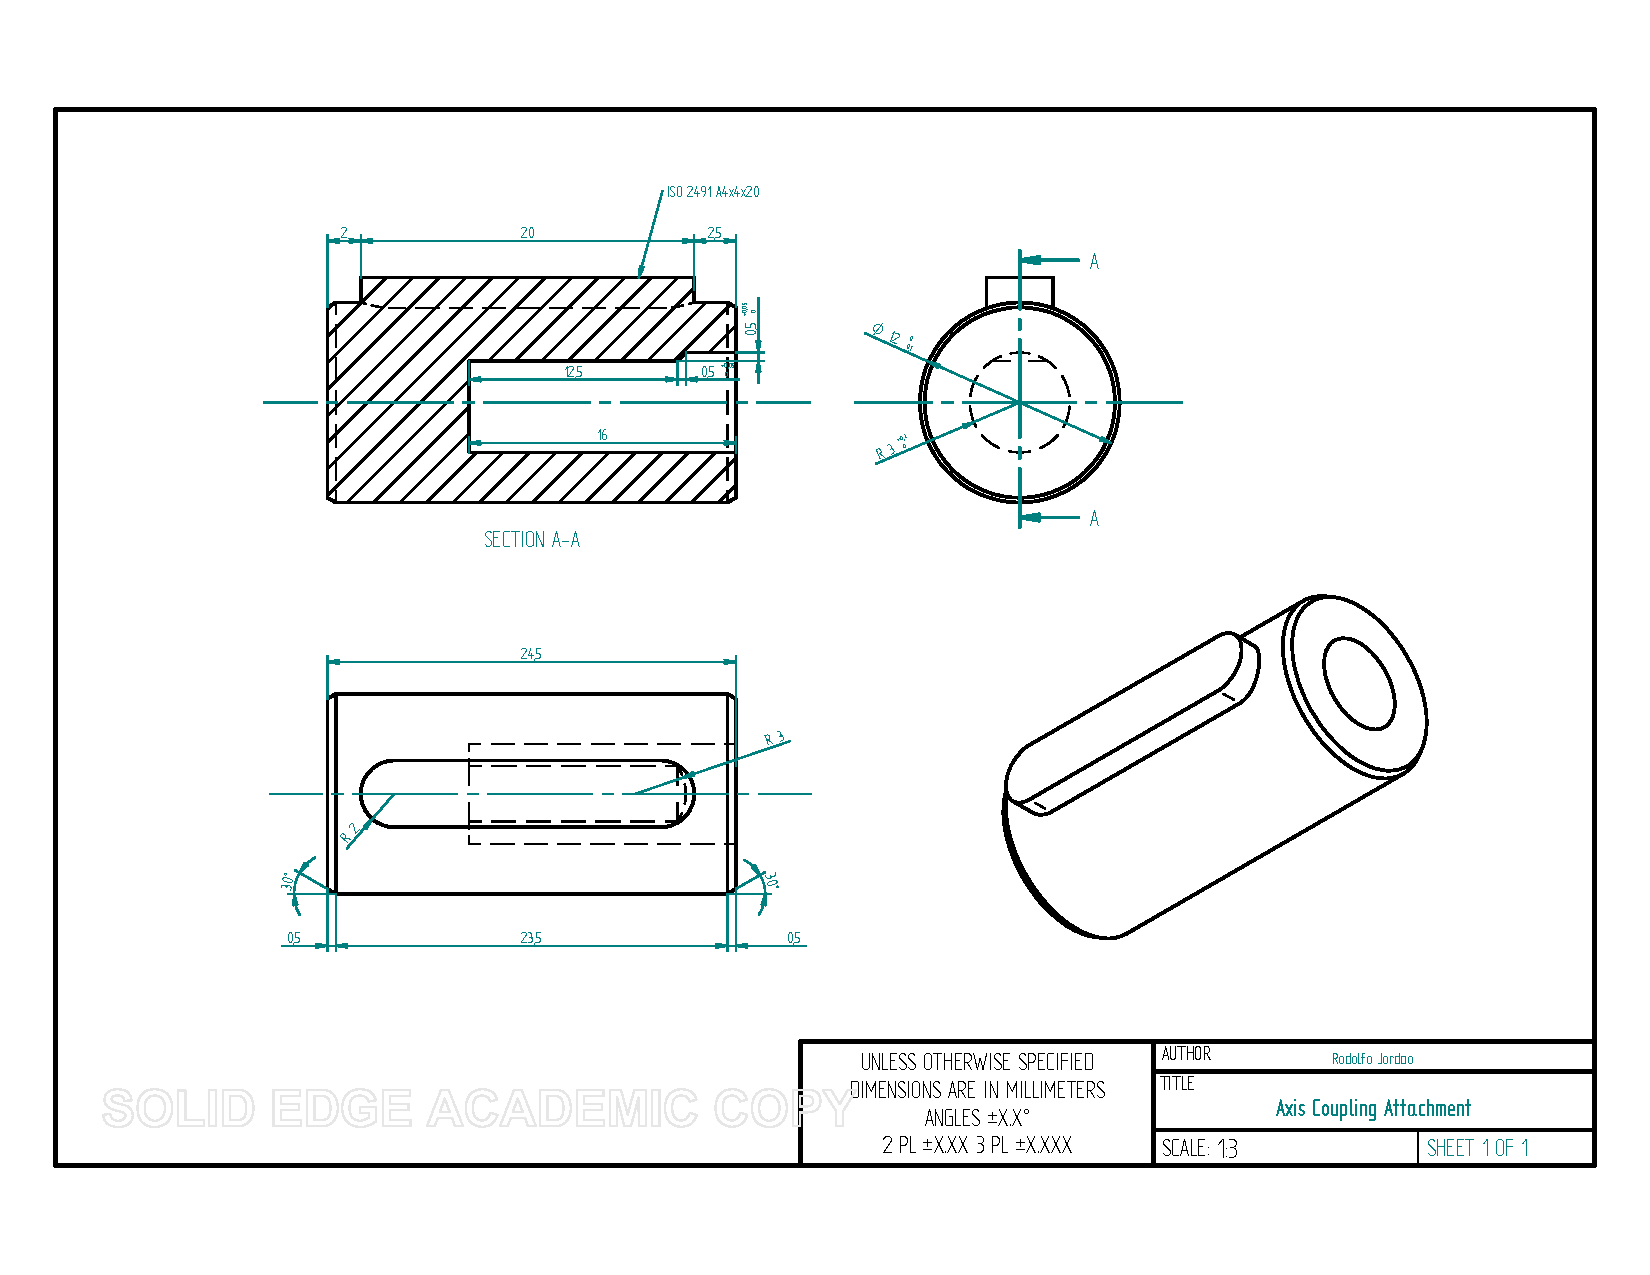
\includegraphics[width=0.9\textwidth]{../CAD/axis}
\end{center}
\caption{Motor axis coupling drawing. \label{fig:axis:draw}}
\end{figure}

\begin{figure}
\begin{center}
% 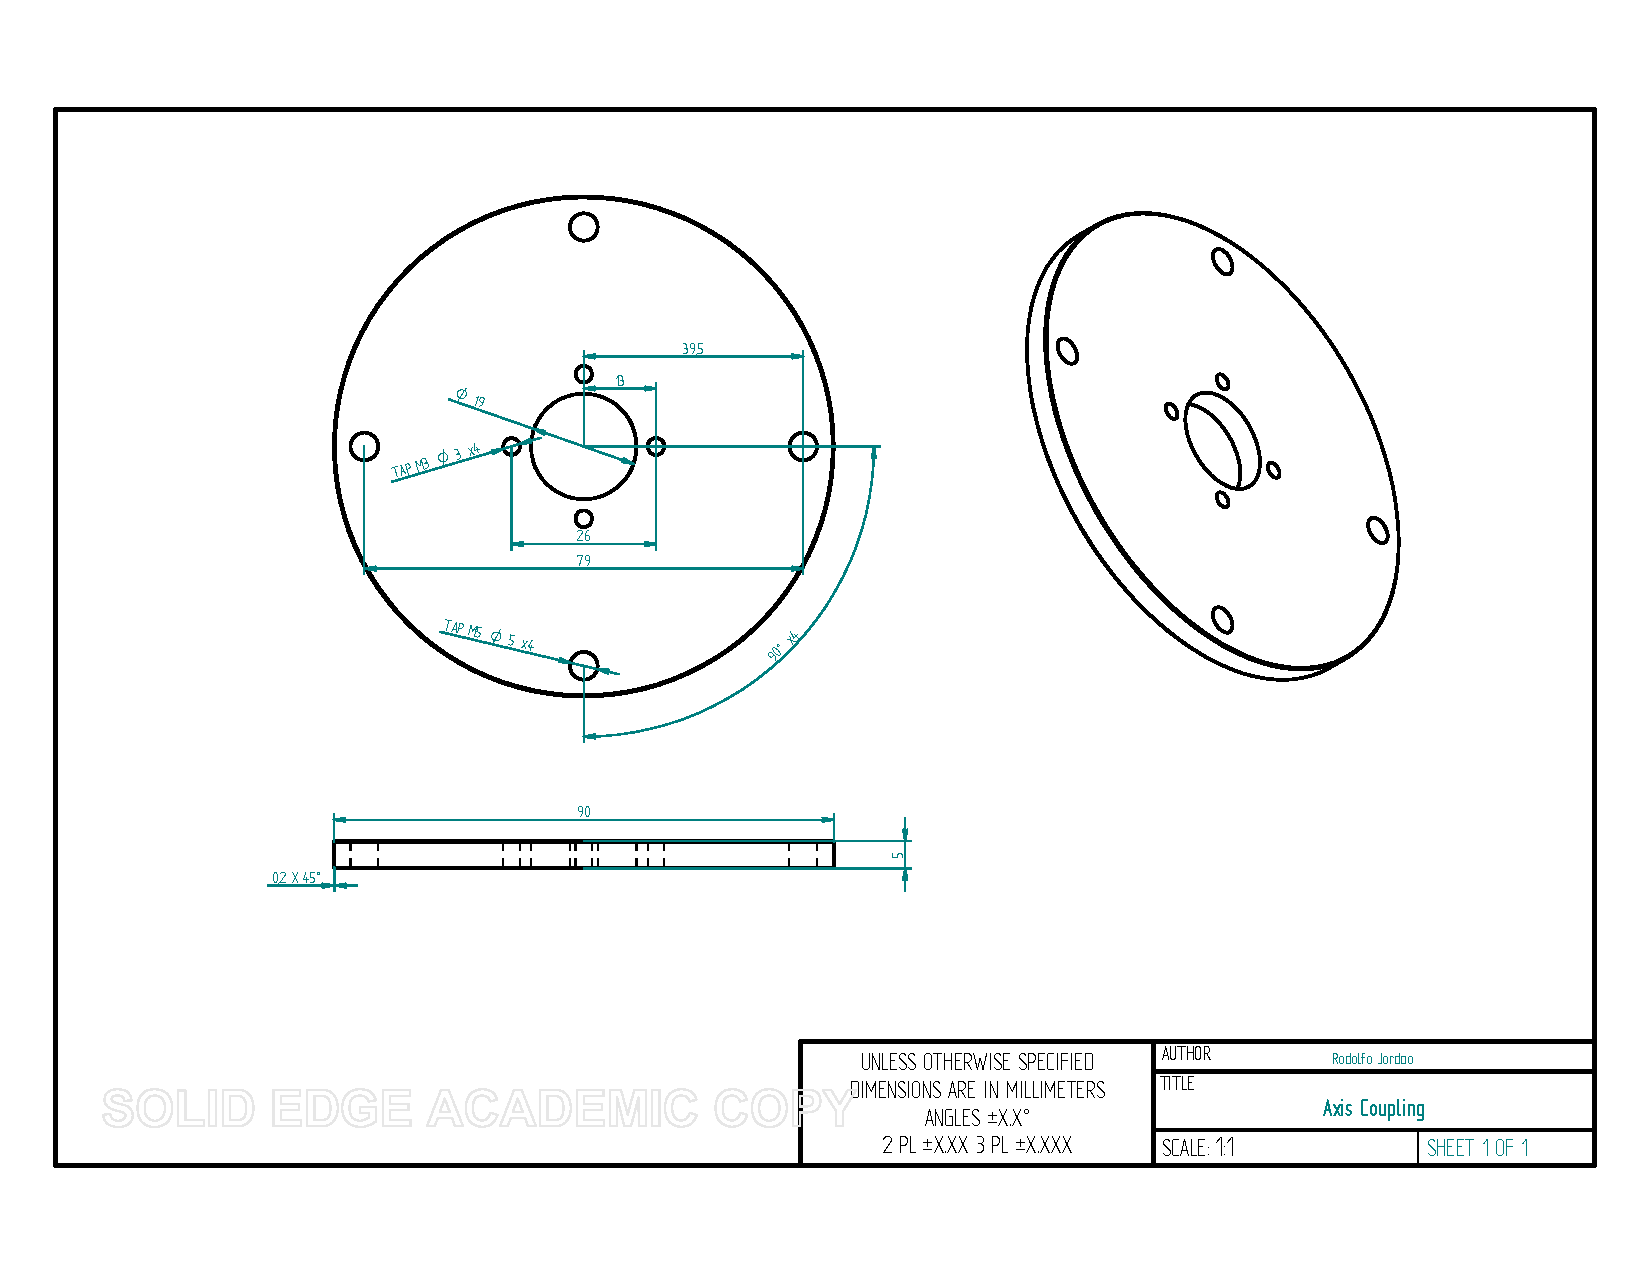
\includegraphics[width=0.9\columnwidth]{../CAD/ring}
\end{center}
\caption{Motor ring coupling drawing. \label{fig:ring:draw}}
\end{figure}

\section{Stall detection\label{sec:stall:detection}}

The implementation is based by the LRS test and will make a check
upon the error of the system is the trend is equilibrium or rising.
The pseudo code is give in Alg.~\ref{alg:stall:detection} while
the implentation is given in Sec.~\ref{chap:arduino:source}.

\begin{algorithm}[h]
\begin{lstlisting}[language=Pascal]
Program Stall_detection
Var error_memory[1..n] : double
If trend of error_memory > 0 Then
	If average of error_memory > error_tolerance Then
		stop motor
Else
	Rerun Stall_detection after sampling
End
\end{lstlisting}
\caption{Error Algorithm. \label{alg:stall:detection}}
\end{algorithm}
care must also be taken to re-initialize the error memory whenever
a new command is issued or a the motor is disabled/enabled. If not,
any test may give wrong predictions.

\section{Computer Interface}

The Graphical Interface is build upon the Qt framework for easy deployment.
A quick picture if it can be seen in Fig.~\ref{fig:interface}.

\begin{figure}[h]
\begin{center}
% 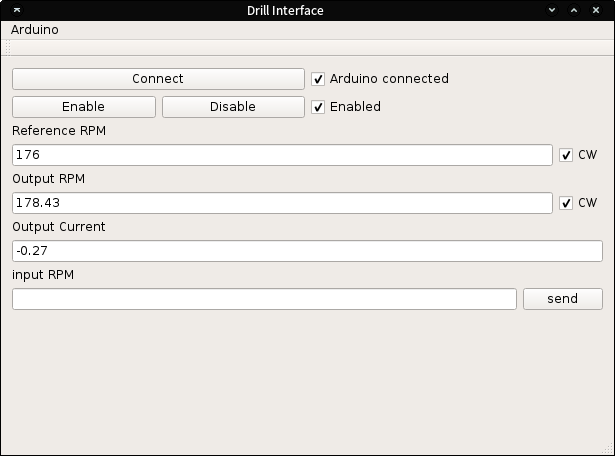
\includegraphics[width=0.6\columnwidth]{../implementation/Interface/screenshot}
\end{center}
\caption{Controller Prototype interface.\label{fig:interface}}
\end{figure}


\bibliography{log}
\bibliographystyle{plain}

\appendix
%
% \chapter{Sagemath Source Code}
% \label{sec:sagemath}
%
% \lstinputlisting[language=Python]{/home/rjordao/Dropbox/SSC_Placement/model.sage}
%
% \chapter{Qt Source Code}
%
% \section{Header file}
%
% \lstinputlisting[language={C++}]{/home/rjordao/Dropbox/SSC_Placement/implementation/Interface/mainwindow.h}
%
% \section{Source file}
%
% \lstinputlisting[language={C++}]{/home/rjordao/Dropbox/SSC_Placement/implementation/Interface/mainwindow.cpp}
%
% \chapter{Arduino Source Code\label{chap:arduino:source}}
%
% \lstinputlisting[language={C++}]{../implementation/Arduino/principal/principal.ino}

\chapter{Deprecated Stuff}

\section{Stall Detection (Deprecated)}

It really depends upon the behavior of the system, but if focus is
mode on the speed error, then some things can be asserted about the
mathematical model:
\begin{defn}[Stall]
	The positive definite error function $e(t)$ is said to be \emph{stalling
		about $L$} if there is $t_{o}\in\R$ such that $\forall t>t_{0},\left|e(t)-L\right|<\epsilon$
	where $\epsilon\in\R$. In words, the error $e(t)$ is \emph{stalling}
	if it oscillates (ou stabilizates) about some value $L$. The discrete
	version is similar.
\end{defn}
Stalling formally defined, it is easier to analyze and develop any
algorithm. In a correct working mechanism, the error will just drop
continuously to zero; hence, in an ideal condition the error function
should be \emph{strictly monotonic deceasing. }The data available
consists of a sequence of real number $\left\{ e(T),\dots,e(nT)\right\} $
sampled approximately at times $kT$, where $k\in\Z$ and $T\in\R$.

now, the behavior of $e(t)$ in respect to time by sampling can be
tracked by many different ways, three based in direct measure, sampled
derivative and sampled integral, respectively, follows:
\begin{prop}[Straight check]
	if $e(nT)\geq e(T)$, then $e(t)$ is not strictly monotonic decreasing
	in the interval.\end{prop}
\begin{proof}
	Follows straight from definition.\end{proof}
\begin{prop}[Ratio integral test]
	if
	\[
	\sum_{i=1}^{N}\frac{e_{i+1}}{e_{i}}\geq N
	\]
	where $e_{i}=e(iT)$, then $e(t)$ is not strictly monotonic decreasing.\end{prop}
\begin{proof}
	Suppose that $e(t)$ is monotonic decreasing and let
	\[
	\sum_{i=1}^{N}\frac{e_{i+1}}{e_{i}}\geq N
	\]
	where $N$ is the size of the sampled set. Now, since $e(t)$ is monotonic
	decreasing,
	\[
	\frac{e_{k+1}}{e_{k}}\leq1\quad\forall k\in\N
	\]
	it follows that,Suppose
	\[
	\sum_{i=1}^{N}\frac{e_{i+1}}{e_{i}}<vectorN
	\]
	which is a contradiction. Thus $e(t)$ cannot be strictly monotonic
	decreasing.\end{proof}
\begin{prop}[Meta integral test]
	let
	\[
	I(a,b)=\sum_{i=a+1}^{b}e_{k}
	\]
	where $a,b\in\N$. If,
	\[
	I(0,N)\leq I(N,2N)
	\]
	then $e(t)$ cannot be strictly monotonic decreasing.\end{prop}
\begin{proof}
	Suppose that $e(t)$ is strictly monotonic decreasing. From definition
	it follows that,
	\[
	e_{k}>e_{k+a}\quad\forall k\in\N
	\]
	where $a\in\N$. Now, summing this inequality with $a=N$ from 1 to
	$N$,
	\[
	I(0,N)=\sum_{i=1}^{N}e_{k}>\sum_{i=1}^{N}e_{k+N}=\sum_{i=N+1}^{2N}e_{k}=I(N,2N)
	\]
	henceforth, if
	\[
	I(0,N)l\leq I(N,2N)
	\]
	a contradiction follows. This completes the proof.
\end{proof}
These propositions can be used to test for stalling of the motor,
since there is a intimate relationship between stalling and a monotonic
decreasing function with error checking. For instance, the error function
by definition should stall at the final error value, as being the
objective; but it should not stall in values greater than the tolerance
for error.
\begin{fact}
	if the error function $e(t)$ is not strictly monotonic decreasing,
	it is either stalling on some value or increasing.
\end{fact}
From this fact, it becomes clear that the checks for a strictly monotonic
decreasing function followed by a check of the total error of the
system returns a safe estimate of its stalling. The actual implementation
can use the three tests as to increase security. This is done at Sec.~\ref{sec:stall:detecion:deprecated}.

\section{Stall detection (deprecated)\label{sec:stall:detecion:deprecated}}

The implementation is rather simple and it's based on simultaneous
tests pass. If more two out of three tests asserts that the system
is possibly stalling, the system is shutdown if the error is above
some tolerance. The code is show in Alg.~\ref{alg:stall:detec} in
pseudo code.

\begin{algorithm}[h]
	\begin{lstlisting}[language=Pascal]
	Program Stall_detection
	Var error_decision: integer
	error_decision := 0
	If straight_error_check is true Then
	error_decision := error_decision + 1
	If ratio_integral_check is true Then
	error_decision := error_decision + 1
	If meta_integral_check is true Then
	error_decision := error_decision + 1
	If error_decision > 2 Then
	stop motor
	Else
	error_decision := 0
	Rerun Stall_detection after sampling
	End
	\end{lstlisting}

	\center{}\protect\caption{Error Algorithm. \label{alg:stall:detec}}
\end{algorithm}

\end{document}
